%-------------------------------------------------------------------------
% Design Project Input/Output Module Description
%-------------------------------------------------------------------------

\clearpage
\section{RF Input Module}
\label{sec-input-rf}

This input module enables your IoT device to send and receive radio
frequency (RF) signals wirelessly in a \wu{25}{ft} radius. RF control
devices are useful in many applications -- e.g., car security systems,
home security and automation systems, garage door controllers, remote
control fan, remote control toys, remote control industrial use. In an
RF-based control system, an RF transmitter emits radio waves in the
range of \wu{3}{kHz} to \wu{300}{GHz}, and an RF receiver receives the
signals and acts on them. In this module, you will use a 4-button keyfob
RF remote to send \wu{315}{MHz} signals to an RF receiver connected to
your Arduino, which can then act on the signal.

A sample circuit is shown below to get you started. The RF receiver
module has seven pins. D0, D1, D2, and D3 are signal pins corresponding
to the four buttons on the keyfob RF remote; VT is a special pin that is
HIGH if any button is pushed and LOW if none are pushed. The 4-button
keyfob RF remote requires no assembly or connectivity. Pressing any of
the four buttons transmits a \wu{315}{MHz} radio wave command that can
be picked up by the RF receiver.

The example Arduino code shown below will read which button you have
pressed on the remote, and then print the output on the serial monitor
every \wu{100}{ms}. After setting up the circuit and programming the
Arduino, open the serial monitor and try pressing each button on the RF
remote. You should see each letter detected by the Arduino displayed on
the serial monitor. Try to see how far away you can move with the RF
remote while still successfully receiving the signal!

\vspace{0.1in}
\begin{minipage}[t]{0.49\tw}

  \vspace{0.0in}
  
\includegraphics[width=\tw]{rf-remote.jpg}

  \vspace{0.0in}
  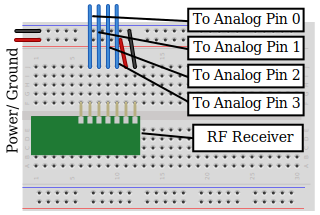
\includegraphics[width=\tw]{input-rf-annotated.svg.pdf}

\end{minipage}
\hfill
\begin{minipage}[t]{0.49\tw}
  \begin{Verbatim}[gobble=3,fontsize=\small]
    int pin_RF_A = 3;
    int pin_RF_B = 6;
    int pin_RF_C = 7;
    int pin_RF_D = 10;

    void setup() {
      pinMode( pin_RF_A, INPUT );
      pinMode( pin_RF_B, INPUT );
      pinMode( pin_RF_C, INPUT );
      pinMode( pin_RF_D, INPUT );
      Serial.begin(9600);
    }

    void loop() {
      // Read RF input on each pin
      int A = digitalRead( pin_RF_A );
      int B = digitalRead( pin_RF_B );
      int C = digitalRead( pin_RF_C );
      int D = digitalRead( pin_RF_D );

      // Print the letter if the input is detected.
      if (A) Serial.print("A"); else Serial.print("-");
      if (B) Serial.print("B"); else Serial.print("-");
      if (C) Serial.print("C"); else Serial.print("-");
      if (D) Serial.print("D"); else Serial.print("-");
      Serial.println(); // make a new line

      // Loop every 100ms.
      delay(100);
    }
  \end{Verbatim}
\end{minipage}
\vspace{0.1in}

%Questions:
